%% ****** Start of file apsguide4-2.tex ****** %
%%
%%   This file is part of the APS files in the REVTeX 4.2 distribution.
%%   Version 4.2b of REVTeX, December 2018.
%%
%%   Copyright (c) 2019 The American Physical Society.
%%
%%   See the REVTeX 4.2 README file for restrictions and more information.
%%
\documentclass[twocolumn,secnumarabic,amssymb, nobibnotes, aps, prd]{revtex4-2}
\usepackage{graphicx} % Required for inserting images
\usepackage{amsmath}
\usepackage{amsfonts}
\usepackage{amsthm}
\usepackage{tikz}
\usetikzlibrary{tikzmark}
\usepackage{braket}
%\usepackage{acrofont}%NOTE: Comment out this line for the release version!
\newcommand{\revtex}{REV\TeX\ }
\newcommand{\classoption}[1]{\texttt{#1}}
\newcommand{\macro}[1]{\texttt{\textbackslash#1}}
\newcommand{\m}[1]{\macro{#1}}
\newcommand{\env}[1]{\texttt{#1}}
\setlength{\textheight}{9.5in}

\begin{document}

\title{A One Way Quantum Computer}%

\author{Yiting Pei}%
\email{yitingpei2029@u.northwestern.edu}
\date{\today}%

\begin{abstract}
    Abstract
\end{abstract}
\maketitle
\tableofcontents

\section{Introduction}

\subsection{Quantum Teleportation}
In this section, I will give a brief summary of quantum teleportation. In the simplest case, quantum teleportation is realized on a $3$-qubit state. Assume that Alice holds two qubit and Bob holds one, and Alice wants to teleport one of her qubit, $\ket{\psi} = \alpha\ket{0} + \beta \ket{1}$ to Bob.\par
First, Alice and Bob entangle their qubits (that is not the one waiting to be teleported) to a maximally entangled state. Then, the three qubit state becomes
\begin{align*}
    \ket{\Psi} = \ket{\psi} \otimes \frac{1}{\sqrt{2}} \left(\ket{0} \otimes \ket{0} + \ket{1} \otimes \ket{1}\right)
\end{align*}
Then, Alice performs a unitary transformation on her two qubits $U = (H \otimes \mathbb{I})CNOT$, the resulting state is
\begin{align*}
    \ket{\Psi'} = \ket{00}\ket{\psi} &+ \ket{01}(\alpha\ket{1} + \beta\ket{0}) \\&+ \ket{10}(\alpha\ket{0} - \beta\ket{1}) + \ket{11}(\alpha\ket{1} - \beta\ket{0})
\end{align*}\par
The input qubit has sucessfully transported to Bob's Hilbert space, with a distortion. However, this distortion can be corrected based on the measurement on Alice's Hilbert space.\par
\begin{itemize}
    \item If Alice has measurement output $\ket{00}$, the qubit is not altered, hence we apply $\mathbb{I}$ on Bob's qubit.
    \item If Alice's measurement output is $\ket{01}$, the qubit experiences a bit flip, hence we apply a $X$ gate on Bob's qubit.
    \item If Alice's measurement output is $\ket{10}$, the qubit experiences a $\pi$ phase shift, so we apply a $Z$ gate on Bob's qubit.
    \item If Alice's measurement output is $\ket{11}$, the qubit experiences both a bit flip and a $\pi$ phase shift. Hence, we apply a $ZX$ gate on Bob's qubit.
\end{itemize}
Combing these three steps, we sucessfully trasport the qubit from Alice's Hilbert space to Bob's Hilbert space without any error.\par

\section{Cluster State}
\subsection{Definition of Cluster State}
To allow the operation of quantum circuit on a lattice of qubits, a cluster state will be needed. Consider an $n$ dimensional lattice of qubits. An $n$-qubit cluster $\mathcal{C}$ is a connected subset of the lattice containing $n$ qubits. Then, the cluster state $\ket{\phi_{\{\kappa\}}}_{\mathcal{C}}$ is direct product of the $n$-qubit state following:
\begin{align}
    K^{(a)} &= \sigma_x^{(a)} \bigotimes_{b \in nbgh(a)} \sigma_z^{(b)} \notag\\
    K^{(a)}\ket{\phi_{\{\kappa\}}}_{\mathcal{C}} &= (-1)^{\kappa_a}\ket{\phi_{\{\kappa\}}}_{\mathcal{C}} \quad \forall a \in \mathcal{C}
\end{align}
where $nbgh(a)$ is the neighborhood of $a$, namely the set of sites that are connected to site $a$, and $\kappa_{a} \in \{0, 1\}$. Further, the set $\{\kappa_a| a \in \mathcal{C}\}$ specifies the cluster state $\ket{\phi_{\{\kappa\}}}_{\mathcal{C}}$. If two cluster states has ${\kappa}$, ${\kappa'}$ different by at least one element, then the two cluster states are orthogonal to each other. Hence, the set of $\{\ket{\phi_{\{\kappa\}}}_{\mathcal{C}} \vert \{\kappa\} \in \{ 0, 1\}^{|\mathcal{C}|} \}$ forms an orthogonal basis of the $2^{|\mathcal{C}|}$ dimensional Hilbert space.\par

\subsection{Preparation}
The first step of create a cluster state on a $\mathcal{C}_n$ cluster is to prepare a product state $\ket{+}_{\mathcal{C}} = \bigotimes_{a \in \mathcal{C}} \ket{+}_a$. Then, apply a unitary transformation
\begin{align}
    S^{(\mathcal{C})} &= \prod_{a,b \in \mathcal{C} | b\in nbgh(a)} S^{ab}\\
    S^{ab} &= \frac{1}{2}\left(1 + \sigma_z^{(a)} + \sigma_z^{(b)} - \sigma_z^{(a)} \otimes \sigma_z^{(b)}\right)\notag
\end{align}
This unitary transformation impose a phase $\pi$ on the state $\ket{1}_a \otimes \ket{1}_b$, and keeps the rest of the states $\ket{0}_a \otimes \ket{0}_b$, $\ket{0}_a \otimes \ket{1}_b$, $\ket{1}_a \otimes \ket{0}_b$ invariant.\par

Following this construction, we can write out the cluster state on 2, 3, 4 qubit cluster.
\begin{align*}
    \ket{\phi_{\{\kappa\}}}_{\mathcal{C}2} &= \frac{1}{\sqrt{2}}\left(\ket{0}_1 \ket{+}_2 + \ket{1}_1\ket{-}_2\right)\\
    \ket{\phi_{\{\kappa\}}}_{\mathcal{C}3} &= \frac{1}{\sqrt{2}}\left(\ket{+}_1 \ket{0}_2 \ket{+}_3 + \ket{-}_1\ket{1}_2\ket{-}_3\right)\\
    \ket{\phi_{\{\kappa\}}}_{\mathcal{C}4} &= \frac{1}{2}(\ket{+}_1 \ket{0}_2 \ket{+}_3\ket{0}_4 + \ket{+}_1 \ket{0}_2 \ket{-}_3\ket{1}_4 \\
    &\ \quad + \ket{-}_1\ket{1}_2\ket{-}_3\ket{0}_4 + \ket{-}_1 \ket{1}_2 \ket{+}_3\ket{1}_4 )
\end{align*}


\section{Construction of Single Quanutm State}
\subsection{CNOT}
\begin{figure}[h!]
    \centering
    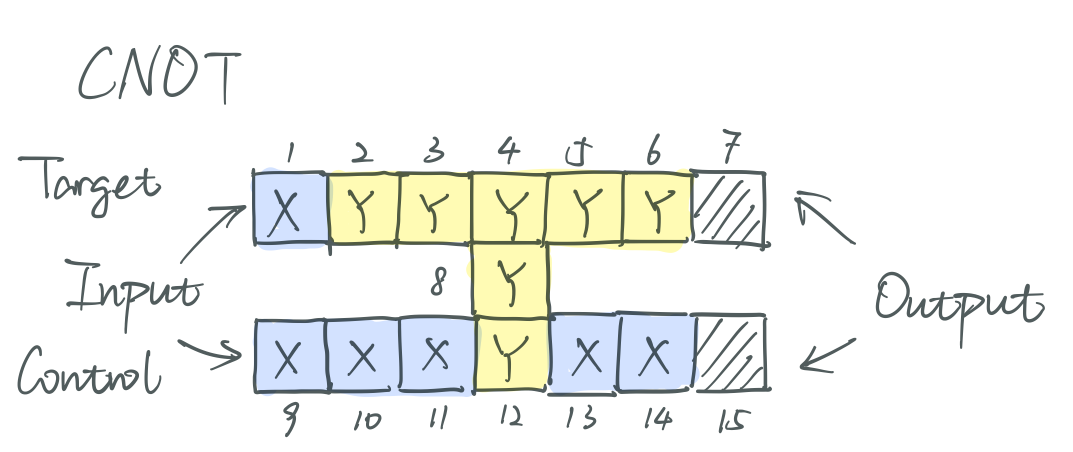
\includegraphics[width=1\linewidth]{CNOT.png}
    \caption{Each box indicates a qubit site. The figure provides the measurement pattern on 15 qubit cluster to realize a CNOT gate.}
    \label{CNOT}
\end{figure}
In this construction, a CNOT gate is realized through a 15 qubit cluster, following the below steps:
\begin{itemize}
    \item Prepare the initial state $\ket{\psi_{in}}_{1,9}\left(\bigotimes_{i\in\mathcal{C}_{15\setminus\{1,9\}}}\ket{+}_i\right)$
    \item Entangle the 15 qubit cluster with the unitary transformation $S^{(\mathcal{C}_{15})}$
    \item One qubit measurement is performed on every qubit in the cluster except for the output qubit(7, 15). The measurement pattern is visualized in Fig.\ref{CNOT}.
    \begin{itemize}
        \item $\sigma_x$ measurement: qubit 1, 9, 10, 11, 13, 14
        \item $\sigma_y$ measurement: qubit 2, 3, 4, 5, 6, 8, 12
        \item The measured qubits would be destroyed and resulting gate is $U'_{CNOT} = U_{\Sigma, CNOT}CNOT(c, t)$
        \item $U_{\Sigma, CNOT} = {\sigma_x^{(c)}}^{\gamma_x^{(c)}}{\sigma_x^{(t)}}^{\gamma_x^{(t)}}{\sigma_z^{(c)}}^{\gamma_z^{(c)}}{\sigma_z^{(t)}}^{\gamma_z^{(t)}} $ with\\
        \begin{align*}
            \gamma_x^{(c)} &= s_2 + s_3 + s_5 + s_6\\
            \gamma_x^{(t)} &= s_2 + s_3 + s_8 + s_{10} + s_{12} + s_{14}\\
            \gamma_z^{(c)} &= s_1 + s_3 + s_4 + s_5 + s_8 + s_9 + s_{11} + 1\\
            \gamma_z^{(t)} &= s_9 + s_{11} + s_{13}
        \end{align*}
    \end{itemize}
\end{itemize}

\subsection{$SU(2)$ Rotation}
\begin{figure}[h!]
    \centering
    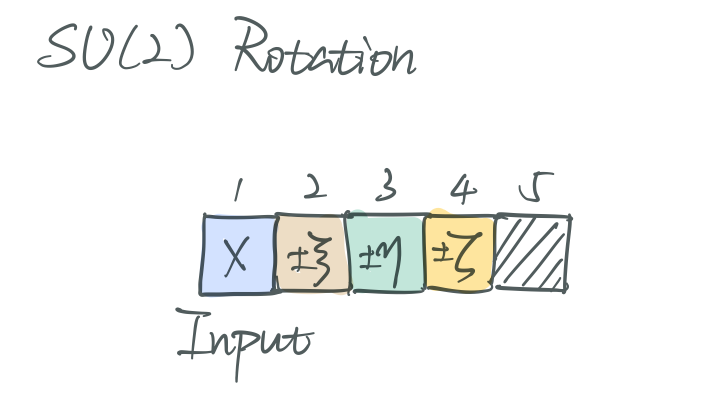
\includegraphics[width=1\linewidth]{Rotation.png}
    \caption{The figure provides the measurement pattern on 5 qubit cluster to realize an arbitrary SU(2) rotation.}
    \label{Rotation}
\end{figure}
Similarly, a general $SU(2)$ rotation can be realized on a 5 qubit cluster. For any $U \in SU(2)$ on a qubit, it can be decomposed into the form $U = U_X[\zeta]U_Z[\eta]U_X[\xi]$, correspond to Euler rotation and its three Euler angles. The procedure is as follow:
\begin{itemize}
        \item Prepare the state $\ket{\Psi}_{\mathcal{C}_5} = \ket{\psi_{in}}_1 \left(\bigotimes_{i = 2}^5 \ket{+}_i\right)$
        \item Create the cluster state by performing the unitary operation $S^{(\mathcal{C}_5)}$
        \item Measure the first 4 qubits in the following order. Each measurement correspond to a step of Euler rotation
            \begin{itemize}
                \item Measure qubit 1 in $\mathcal{B}_1(0)$.
                \item Measure qubit 2 in $\mathcal{B}_2(-\xi(-1)^{s_1})$.
                \item Measure qubit 3 in $\mathcal{B}_3(-\eta(-1)^{s_2})$.
                \item Measure qubit 4 in $\mathcal{B}_4(-\zeta(-1)^{s_2+s_3})$.
            \end{itemize}
        With $\mathcal{B}_j(\varphi_j) = \Bigl\{\frac{\ket{0}_i + e^{i\varphi}\ket{1}_j}{\sqrt{2}},\frac{\ket{0}_i - e^{i\varphi}\ket{1}_j}{\sqrt{2}} \Bigr\}$
        \item Then, we have performed a rotation $U'_{Rot} = U_{\Sigma,Rot}U_{Rot}[\eta, \xi, \zeta]$, with the byproduct operator $U_{\Sigma,Rot} = \sigma_x^{s_2+s_4}\sigma_z^{s_1+s_3}$
    \end{itemize}


\subsection{Hadamard and $\pi/2$-Phase Gate}
\begin{figure}[h!]
    \centering
    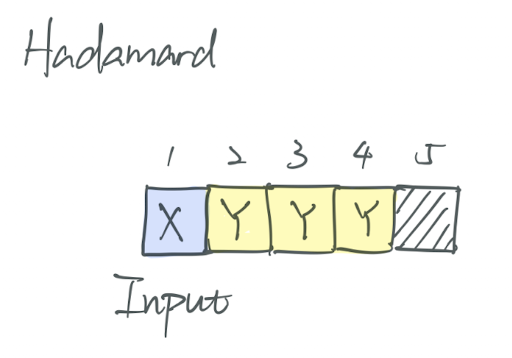
\includegraphics[width=1\linewidth]{Hadamard.png}
    \caption{The figure provides the measurement pattern on 5 qubit cluster to realize an arbitrary Hadamard Gate.}
    \label{Hadamard}
\end{figure}
\begin{figure}[h!]
    \centering
    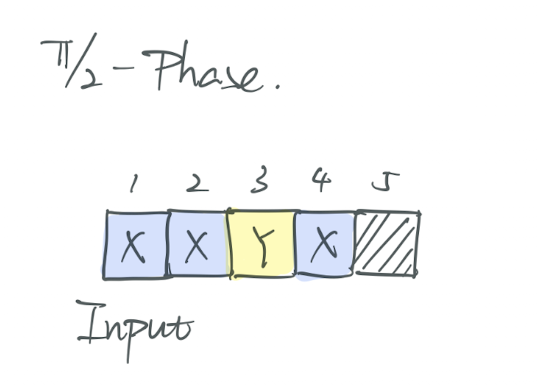
\includegraphics[width=1\linewidth]{Pi2.png}
    \caption{The figure provides the measurement pattern on 5 qubit cluster to realize an arbitrary $\pi/2$-phase gate.}
    \label{Pi2}
\end{figure}
In the previous section, I described the scheme to construct the measurement pattern for a general $SU(2)$ rotation. The measurement must be performed in the order specified. However, there is a special class of single qubit gates where the measurement can be performed simultaneously. In this section, I will give two examples of such gates, Hadamard gate and $\pi/2$-phase gate.\par

Both gates are constructed on a 5-qubit cluster. 
\begin{itemize}
    \item Prepare the 5-qubit cluster state
    \item Measurement of the first 4 qubit can be performed simultaneously
    \begin{itemize}
        \item Hadamard Gate: $\sigma_x^{(1)}$, $\sigma_y^{(2)}$, $\sigma_y^{(3)}$, $\sigma_y^{(4)}$, $U_{\Sigma, H} = \sigma_x^{s_1+s_3+s_4}\sigma_z^{s_2+s_3}$
        \item $\pi/2$-phase Gate: $\sigma_x^{(1)}$, $\sigma_x^{(2)}$, $\sigma_y^{(3)}$, $\sigma_x^{(4)}$, $U_{\Sigma, H} = \sigma_x^{s_2+s_4}\sigma_z^{s_1+s_2+s_3+1}$.
    \end{itemize}
\end{itemize}

\section{Quantum Circuit: Logical Network}
\begin{figure*}
    \centering
    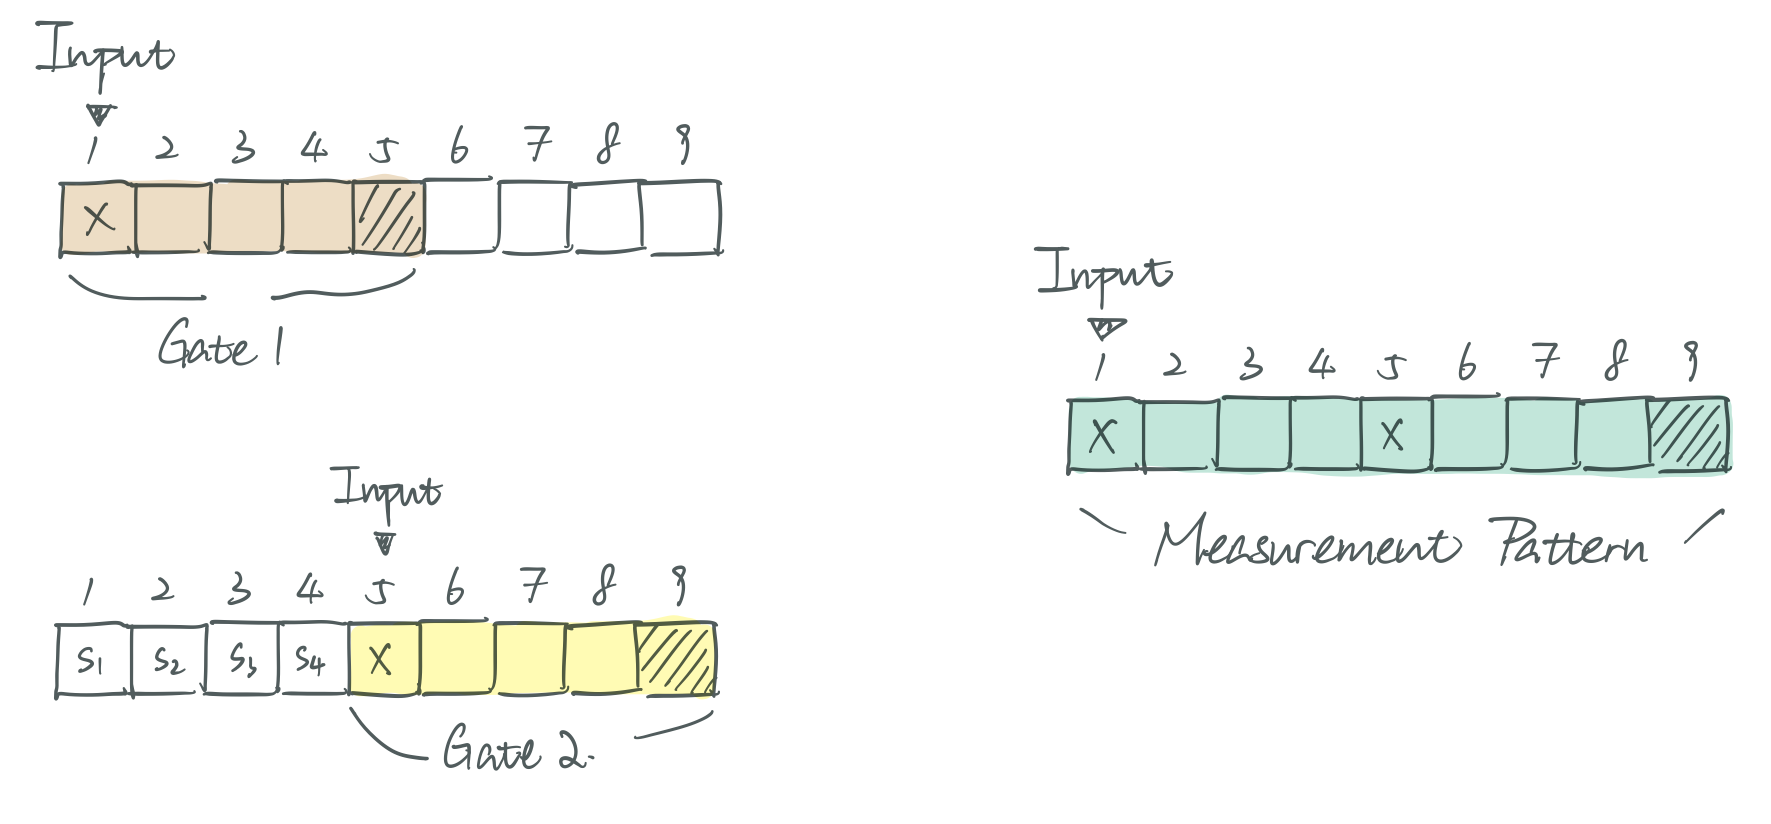
\includegraphics[width=1\linewidth]{Logical Network.png}
    \caption{}
    \label{Logical Network}
\end{figure*}

\section{Conclusion}

\end{document}

